\chapter{Methodology}\label{chapter-2.-methodology}

This chapter describes the technical design of the system. Section 2.1 gives a top-level view of the architecture and the data flow from the raw satellite image to the final inventory. Sections 2.2 through 2.7 detail the four detection models proposed in the literature gap of Chapter 1 --- YOLOv8-seg, Mask R-CNN, DeepForest, and SAM 2 --- and the ensemble strategy of Section 2.8 that combines their detector outputs. Sections 2.9 and 2.10 cover the geographic conversion of pixel coordinates to longitude / latitude and the export of the inventory in formats consumable by GIS specialists. Implementation choices and trade-offs are justified throughout.

\section{System architecture overview}\label{system-architecture-overview}

The proposed system follows a classical three-tier separation of concerns: a thin \textbf{presentation layer} (a single-page React 18 application served via CDN-loaded UMD bundles and rendered with Babel-standalone), an \textbf{application layer} (a FastAPI REST backend implemented in Python 3.11) and a \textbf{model layer} (three deep-learning adapters that wrap the underlying frameworks --- Ultralytics YOLO for YOLOv8-seg, the DeepForest library for the RetinaNet-based detector and the official SAM 2 implementation from Meta AI for the mask-refinement stage).

The data flow through the system can be summarised as follows:

\begin{enumerate}
\def\labelenumi{\arabic{enumi}.}
\tightlist
\item
  The user opens the web interface and either uploads a satellite image as a file (PNG, JPG, TIFF or GeoTIFF) or selects an area directly on a Leaflet map; in the latter case the backend downloads the appropriate ESRI World Imagery tiles, stitches and crops them, and returns the resulting image with embedded geographic bounds.
\item
  The image is stored on the server and assigned an opaque identifier. Image dimensions and, if available, GeoTIFF projection metadata are extracted via the \texttt{rasterio} library.
\item
  The user selects one of three detection backends (YOLO, DeepForest, Ensemble) and a confidence threshold, and triggers inference. The corresponding adapter is loaded lazily on first request and reused for subsequent calls.
\item
  For images larger than the network's native input resolution, the adapter performs sliding-window tiled inference, runs the model on each tile and aggregates the per-tile predictions through Non-Maximum Suppression to produce a single global set of detections.
\item
  Each detection is annotated with geographic coordinates via the geographic-conversion module, which supports four operating modes depending on the metadata available (GeoTIFF affine transform, four-corner bilinear interpolation, two-corner axis-aligned conversion, or no conversion).
\item
  The result is stored as an immutable job record, returned to the frontend for interactive visualisation on a Leaflet map, and made available for export in three formats (GeoJSON, CSV, standalone HTML).
\end{enumerate}

A key architectural decision is the use of the \textbf{adapter pattern} for the model layer: every model adheres to a single abstract base class with a \texttt{predict(image\_path,\ confidence)\ -\textgreater{}\ List{[}Detection{]}} method, so that new models can be added without changes to the rest of the system. The base class also provides lazy initialisation, automatic weight loading from a dedicated \texttt{weights/} directory, and exception conversion to FastAPI HTTP responses.

The technology stack and the responsibilities of each component are summarised in Table 2.1.

\textbf{Table 2.1 --- Technology stack of the proposed system.}

{\def\LTcaptype{none} % do not increment counter
\begin{longtable}[]{@{}
  >{\raggedright\arraybackslash}p{(\linewidth - 4\tabcolsep) * \real{0.3333}}
  >{\raggedright\arraybackslash}p{(\linewidth - 4\tabcolsep) * \real{0.3333}}
  >{\raggedright\arraybackslash}p{(\linewidth - 4\tabcolsep) * \real{0.3333}}@{}}
\toprule\noalign{}
\begin{minipage}[b]{\linewidth}\raggedright
Component
\end{minipage} & \begin{minipage}[b]{\linewidth}\raggedright
Technology
\end{minipage} & \begin{minipage}[b]{\linewidth}\raggedright
Responsibility
\end{minipage} \\
\midrule\noalign{}
\endhead
\bottomrule\noalign{}
\endlastfoot
Frontend & React 18 (UMD), Leaflet, Babel-standalone & Drag-and-drop upload, interactive map, statistics, export buttons \\
Backend & FastAPI, Pydantic, Uvicorn & REST API, request validation, lazy model loading \\
Persistence & SQLite (\texttt{storage/app.db}) & Snapshots, runs, detections (3 tables, cascading FK) \\
Geo & rasterio, NumPy, Shapely & GeoTIFF parsing, pixel-to-geo conversion, polygon clipping \\
Model --- YOLO & Ultralytics YOLO 8.4, PyTorch 2.5 + CUDA 12.1 & Instance segmentation of tree crowns \\
Model --- DeepForest & DeepForest 1.5 (RetinaNet) & Bounding-box detection of tree crowns \\
Model --- Mask R-CNN & Detectron2 / torchvision (ResNet-50 + FPN) & Instance segmentation of tree crowns (architectural alternative to YOLO) \\
Model --- SAM 2 & sam2 1.1 (hiera-base-plus) & Zero-shot mask refinement of DeepForest boxes \\
Ensemble & ensemble-boxes (Weighted Box Fusion) & Score-weighted combination of YOLO and DeepForest predictions \\
Map capture & urllib + Pillow (PIL) & ESRI World Imagery tile download, stitching, crop to bbox \\
Export & Custom serialisers + Leaflet HTML template & GeoJSON / CSV / standalone HTML output \\
\end{longtable}
}

The complete source tree of the prototype is organised in three top-level directories --- \texttt{backend/}, \texttt{frontend/} and \texttt{ml/} --- and is approximately 6 000 lines of code. The training and dataset-preparation scripts in \texttt{ml/} are independent from the backend and can be run on a separate machine.

The system architecture follows a three-tier separation of concerns: the React 18 + Leaflet frontend communicates with the FastAPI backend via REST, which in turn dispatches inference requests to one of four pluggable model adapters (YOLOv8-seg, Mask R-CNN, DeepForest, DeepForest+SAM 2). Results are persisted in an SQLite database and returned to the frontend for interactive visualisation and export.

The complete data flow from user-drawn rectangle to exported inventory is summarised in Figure 2.1.

\begin{verbatim}
   ┌─────────────────────────────────────────────────────────────────────┐
   │  PRESENTATION LAYER  (React 18 UMD + Leaflet, no build step)        │
   │  ┌────────────────────────────────────────────────────────────────┐ │
   │  │  Single-image view  │  City-map view  │  Scan area / Polygon   │ │
   │  └────────────────────────────────────────────────────────────────┘ │
   └──────────────────────────────────┬──────────────────────────────────┘
                                      │ HTTP / NDJSON streaming
   ┌──────────────────────────────────▼──────────────────────────────────┐
   │  APPLICATION LAYER  (FastAPI + Pydantic, Python 3.12)               │
   │                                                                     │
   │   /api/upload       /api/capture_from_map      /api/scan_region    │
   │   /api/predict      /api/scan_region/stream    /api/export/...     │
   │                                                                     │
   │   ┌────────────────┐   ┌───────────────────┐   ┌────────────────┐  │
   │   │  Map capture   │   │  Region scanner   │   │   Geo module   │  │
   │   │ (ESRI/Google)  │   │ (3-level tiling)  │   │ (4 geo modes)  │  │
   │   └────────────────┘   └───────────────────┘   └────────────────┘  │
   │                                                                     │
   └────────┬───────────────┬───────────────┬──────────────┬─────────────┘
            │               │               │              │
   ┌────────▼─────┐ ┌───────▼────────┐ ┌────▼─────────┐ ┌──▼─────────────┐
   │   YOLO       │ │  Mask R-CNN    │ │  DeepForest  │ │  DeepForest +  │
   │   adapter    │ │  adapter       │ │  adapter     │ │  SAM 2 adapter │
   │ (Ultralytics)│ │ (torchvision)  │ │ (deepforest) │ │ (sam2 1.1)     │
   └────────┬─────┘ └───────┬────────┘ └──────┬───────┘ └────────┬───────┘
            └───────────────┴────────────┬────┴──────────────────┘
                                         │
                              ┌──────────▼──────────┐
                              │  Weighted Box       │
                              │  Fusion ensemble    │
                              │  (YOLO + DF)        │
                              └──────────┬──────────┘
                                         │ List<Detection>
   ┌─────────────────────────────────────▼─────────────────────────────────┐
   │  PERSISTENCE LAYER  (SQLite, storage/app.db, ON DELETE CASCADE)       │
   │                                                                       │
   │   ┌─────────────┐    ┌────────────┐    ┌──────────────────────┐       │
   │   │ snapshots   │◄───┤   runs     │◄───┤    detections        │       │
   │   └─────────────┘    └────────────┘    └──────────────────────┘       │
   │                            ▲                                          │
   │                     ┌──────┴──────┐                                   │
   │                     │ scan_sessions│                                  │
   │                     └─────────────┘                                   │
   └───────────────────────────────────────────────────────────────────────┘
                                         │
   ┌─────────────────────────────────────▼─────────────────────────────────┐
   │  EXPORT LAYER                                                         │
   │  ┌─────────────┐    ┌──────────────┐    ┌──────────────────────────┐  │
   │  │  GeoJSON    │    │     CSV      │    │  Standalone HTML (Leaflet)│  │
   │  └─────────────┘    └──────────────┘    └──────────────────────────┘  │
   └───────────────────────────────────────────────────────────────────────┘
\end{verbatim}

\textbf{Figure 2.1 --- Layered architecture of the proposed system.} Solid arrows denote a synchronous request / response; the ON-DELETE-CASCADE relations between SQLite tables ensure that deleting a snapshot or a scan-session also removes all dependent runs, detections and PNG files in a single operation.

\section{Image input and pre-processing}\label{image-input-and-pre-processing}

The system accepts three categories of input, each with its own pre-processing path.

\textbf{Regular images} (PNG, JPG, WebP) are stored as-is and decoded with Pillow on the first call. The width and height are recorded as part of the image metadata. Such images carry no geographic information, and the user is expected to supply geographic anchors manually --- either as two corners (north-west and south-east) or as four corners (one per image corner) --- through draggable markers on the map widget.

\textbf{GeoTIFF images} carry an affine transform and a coordinate reference system in their internal metadata. The backend parses this metadata with \texttt{rasterio.open()} and extracts the bounds in WGS-84 (EPSG:4326). For GeoTIFFs in other projections (a common case for satellite data delivered in UTM zones) the bounds are re-projected with \texttt{pyproj}. This path is the most accurate and is the recommended workflow for final, reproducible inventories.

\textbf{In-browser map capture} is the third option, designed for the user who has neither a pre-downloaded GeoTIFF nor a screenshot but wants to inspect a specific area of the city interactively. The user draws a rectangle on a Leaflet map and submits the request to the \texttt{/api/capture\_from\_map} endpoint (single-shot capture) or, more commonly, to \texttt{/api/scan\_region} for an \emph{Auto-Zoom Region Scan} that automatically subdivides a larger bounding box into a grid of sub-regions at a fixed zoom level of 19. The backend then:

\begin{enumerate}
\def\labelenumi{\arabic{enumi}.}
\tightlist
\item
  Converts the two corner coordinates from longitude / latitude into floating-point tile coordinates using the Web-Mercator projection: \(x = (\lambda + 180) / 360 \cdot 2^z\) and \(y = (1 - \log(\tan\phi + \sec\phi) / \pi) / 2 \cdot 2^z\), where \(z\) is the zoom level.
\item
  Computes the integer range of tiles that must be downloaded to cover the requested bounding box and, for large bounding boxes, splits the region into a grid of up to nine sub-bounding-boxes each capped at approximately 100 tiles, so the resulting per-tile downloads remain below a configurable \texttt{MAX\_TILES} limit (default 400, ≈ 5 120 × 5 120 pixels per sub-region) that protects the server from accidental bulk downloads and out-of-memory failures.
\item
  Downloads the tiles in parallel through a thread pool of eight workers from the chosen tile provider. Two providers are currently registered (Table 2.1a): the default \textbf{ESRI World Imagery} endpoint (max zoom 19, no API key required, stable) and an unofficial \textbf{Google Satellite} endpoint (max zoom 20, the same image base as Google Earth Pro --- directly relevant because the YOLO and Mask R-CNN training data is composed of Google Earth Pro screenshots). The provider is selected per request through the optional \texttt{provider} field of the JSON body. Failed tiles are replaced by a small grey placeholder so that a single missing tile does not invalidate the entire capture.
\item
  Stitches the tiles into a single canvas, crops the canvas to the exact bounding box (using the fractional part of the original tile coordinates as sub-tile offsets) and returns a PNG image with the geographic bounds embedded as part of the response. For multi-region scans each sub-region is persisted as an independent snapshot in the SQLite database (Section 2.10) and tagged with the parent scan-session identifier so that the user can later delete the entire scan in a single operation.
\end{enumerate}

\textbf{Table 2.1a --- Tile providers registered in \texttt{backend/map\_capture.py::TILE\_PROVIDERS}.}

{\def\LTcaptype{none} % do not increment counter
\begin{longtable}[]{@{}
  >{\raggedright\arraybackslash}p{(\linewidth - 6\tabcolsep) * \real{0.2500}}
  >{\raggedright\arraybackslash}p{(\linewidth - 6\tabcolsep) * \real{0.2500}}
  >{\raggedright\arraybackslash}p{(\linewidth - 6\tabcolsep) * \real{0.2500}}
  >{\raggedright\arraybackslash}p{(\linewidth - 6\tabcolsep) * \real{0.2500}}@{}}
\toprule\noalign{}
\begin{minipage}[b]{\linewidth}\raggedright
Provider key
\end{minipage} & \begin{minipage}[b]{\linewidth}\raggedright
Endpoint
\end{minipage} & \begin{minipage}[b]{\linewidth}\raggedright
Max zoom
\end{minipage} & \begin{minipage}[b]{\linewidth}\raggedright
Notes
\end{minipage} \\
\midrule\noalign{}
\endhead
\bottomrule\noalign{}
\endlastfoot
\texttt{esri} (default) & \texttt{server.arcgisonline.com/.../World\_Imagery/...} & 19 & Free, no API key, stable \\
\texttt{google} & \texttt{mt\{0–3\}.google.com/vt/lyrs=s} & 20 & Same image base as Google Earth Pro (training data source); unofficial endpoint, used for academic prototyping only \\
\end{longtable}
}

Subsequent inference on the captured image proceeds as if the user had uploaded a GeoTIFF --- the two corners are known with sub-pixel precision and the conversion module switches automatically into two-corner axis-aligned mode.

For all three input categories the maximum file size is currently limited to 100 MiB and the supported extensions are \texttt{.png}, \texttt{.jpg}, \texttt{.jpeg}, \texttt{.tif}, \texttt{.tiff} and \texttt{.webp}.

\section{Tiled processing of high-resolution images}\label{tiled-processing-of-high-resolution-images}

A central design challenge of the system is the \textbf{scale mismatch} between the typical satellite image and the input resolution of the underlying networks. A YOLOv8-seg or DeepForest model operates on inputs of approximately 640 × 640 pixels; a single satellite screenshot of a city block, however, is often 1 600 × 1 100 pixels or larger. If such an image were resized to fit the network's input, each individual tree crown --- typically 20 -- 40 pixels in diameter at zoom 18 --- would shrink to fewer than ten pixels, well below the resolution that any modern detector can reliably handle. This effect was confirmed empirically in early experiments: a YOLOv8-seg model trained at imgsz=640 directly on the full-resolution inputs detected zero trees on the validation set.

The proposed solution is \textbf{sliding-window tiled inference} at the same resolution as training. The original image is partitioned into overlapping tiles of fixed size (640 pixels) with an overlap region (128 pixels) on each side, so that any tree crown is fully contained in at least one tile. The model is then applied independently to each tile and the per-tile detections are translated back into the global image coordinate system by adding the tile offset to every polygon vertex and bounding-box coordinate.

To remove duplicate detections of the same tree that appears in two or more overlapping tiles, the system applies \textbf{global Non-Maximum Suppression} with an IoU threshold of 0.5. The procedure is vectorised in NumPy and operates on the full set of global bounding boxes, sorting by confidence and iteratively discarding any box that overlaps a higher-confidence box above the threshold.

The same tiling-and-NMS pattern is used in three places: in \texttt{predict\_tiled()} inside the YOLO adapter at inference time; in the dataset-preparation script (\texttt{ml/tile\_dataset.py}) that re-tiles the training data; and in the pre-labelling tool (\texttt{ml/prelabel\_coco.py}) that uses the v1 model to generate pre-annotations for new images.

\section{YOLOv8-seg branch}\label{yolov8-seg-branch}

\subsection{Architecture}\label{architecture}

YOLOv8 {[}32{]} is a single-stage anchor-free object detector that operates as a fully-convolutional network with a CSP-Darknet53 backbone, a Path Aggregation Network neck and three detection heads producing predictions at three scales (down-sampling factors of 8, 16 and 32). The segmentation variant \texttt{YOLOv8x-seg} extends this architecture with an additional \textbf{prototype mask head} that produces 32 prototype masks at one quarter the input resolution; each detected instance is then represented by a vector of 32 coefficients that, when linearly combined with the prototype masks and thresholded, produce a binary segmentation mask aligned with the detected bounding box. This design --- borrowed from the YOLACT family of real-time instance segmenters --- separates the per-pixel and the per-instance computations, so the cost of generating masks scales with the number of detections rather than with the number of pixels.

Three YOLOv8-seg variants are used in this work, corresponding to the three phases of the project's hyperparameter ablation reported in Chapter 3. The pre-ablation generations (Sections 3.3.1 -- 3.3.6) used \texttt{yolov8x-seg} --- the largest variant, approximately 71 million parameters --- on the initial hypothesis that the extra capacity would improve performance on the small, moderately-noisy polygon dataset. Rounds 1 -- 3 of the systematic ablation (Section 3.3.7) reversed that hypothesis with the medium-size \texttt{yolov8m-seg} (approximately 27 M parameters) outperforming both larger variants by 15 -- 25 \% relative on Box mAP@50 when trained from COCO weights with manually-tuned (v2-proven) augmentation. Round 4 (Section 3.3.8) then reversed the reversal: with \textbf{Ultralytics' default augmentation pipeline} instead of the manually-tuned one, the largest \texttt{yolov8x-seg} variant once again becomes the strongest single configuration, reaching Box mAP@50 = 0.315 on M14 --- the headline empirical result of the diploma. The \textbf{final production checkpoint} is therefore \texttt{yolov8x-seg} trained from fresh COCO weights with \texttt{single\_cls=True} and Ultralytics' default augmentation (aggressive HSV colour jitter, random erasing, zero geometric transformations). The intermediate \texttt{yolov8m-seg} variant of Round 1 remains in the project's archive under \texttt{weights/v3\_runs/exp1\_m\_cocostart\_*.pt} as a member of the cross-YOLO voting ensemble of Section 2.8.2 below.

\subsection{Why instance segmentation rather than detection}\label{why-instance-segmentation-rather-than-detection}

Bounding-box detection is sufficient for counting trees but is poorly suited to the downstream tasks expected from the system. The municipal user is interested not only in the number of trees but also in their \textbf{crown size}, which is a proxy for both species and age, and in the \textbf{green-coverage percentage} of a given area, which is a standard indicator in urban-planning regulations. Both quantities require pixel-level masks rather than rectangular boxes --- a poplar tree and a birch tree of the same canopy area can have radically different crown silhouettes, and the rectangular bounding box of two adjacent overlapping trees can cover an area that includes a substantial fraction of bare ground.

For these reasons the YOLO branch of the system performs full instance segmentation. The output of the adapter is a list of objects each containing: a bounding box, a polygon mask (the YOLO mask compressed into a closed sequence of \((x, y)\) vertices via Suzuki--Abe contour extraction), a confidence score, and --- derived from the mask --- the crown area in pixels and (if pixel size in metres is known) in square metres.

\subsection{Training data and pre-processing}\label{training-data-and-pre-processing}

The training data for the YOLO branch is a collection of satellite screenshots of Astana taken from Google Earth and ESRI World Imagery at zoom levels 17 to 19. The annotation effort proceeded in two iterations.

\textbf{Version 1} (April 2026): 20 source images were annotated manually in CVAT, producing 2 242 individual tree polygons. The class taxonomy was deliberately kept minimal --- a single class ``Tree'' (in the source: ``Дерево'') --- because the satellite resolution available does not allow reliable species discrimination. The dataset was split into 16 training images and 4 validation images at the source-image level (so that no tile from a single source can leak between splits) and tiled into 62 tiles of 640 × 640 pixels with 128-pixel overlap, of which 58 were used for training and 4 for validation. After the polygon-clipping and minimum-area filtering performed by the tiler, the resulting tiled dataset contained 4 628 polygons.

\textbf{Version 2} (May 2026, current): 57 additional source images were collected and pre-labelled with the v1 model through the iterative tool described in section 2.3, producing a coarse first pass that was then manually refined in CVAT. The new annotations were merged with the version-1 annotations through a custom COCO-merge script that re-numbers \texttt{image\_id} and \texttt{annotation\_id} to avoid collisions while de-duplicating overlapping filenames. The combined dataset contains approximately 77 source images and, after tiling, approximately 5 000 polygon-level annotations distributed over 111 training tiles and 10 validation tiles.

Two custom Python tools support this workflow. \texttt{ml/coco\_to\_yolo\_seg.py} converts a CVAT-exported COCO 1.0 annotation file into the polygon-line format expected by Ultralytics YOLO, with sanitisation of Cyrillic filenames into ASCII to avoid Windows-path issues, an explicit duplicate-policy flag for images shared between train and val splits, and explicit handling of the Cyrillic class name. \texttt{ml/tile\_dataset.py} performs the sliding-window tiling itself using Shapely for polygon clipping, dropping any clipped fragment whose area falls below 25 square pixels (the assumption being that a tree fragment that small is more likely to be an artefact than a useful training signal).

\subsection{Training procedure}\label{training-procedure}

The training of the v1 model was performed on a single workstation with an Intel Core i7-13620H CPU, 16 GiB of system RAM and an NVIDIA GeForce RTX 4060 Laptop GPU with 8 GiB of VRAM. The hyper-parameters are listed in Table 2.2.

\textbf{Table 2.2 --- Training hyper-parameters for the YOLOv8-seg v1 run.}

{\def\LTcaptype{none} % do not increment counter
\begin{longtable}[]{@{}ll@{}}
\toprule\noalign{}
Parameter & Value \\
\midrule\noalign{}
\endhead
\bottomrule\noalign{}
\endlastfoot
Base model & \texttt{yolov8x-seg.pt} (COCO pre-trained) \\
Input resolution & 640 × 640 \\
Batch size & 2 \\
Epochs (max) & 500 \\
Early-stopping patience & 100 \\
Optimiser & AdamW (auto-selected by Ultralytics) \\
Initial learning rate & 0.01 (decayed with cosine schedule) \\
Box loss weight & 7.5 \\
Classification loss weight & 0.5 \\
DFL loss weight & 1.5 \\
Mosaic augmentation & 1.0 \\
Mix-up augmentation & 0.1 \\
Copy-paste augmentation & 0.1 \\
HSV-S / HSV-V jitter & 0.4 / 0.3 \\
Rotation jitter & ±20° \\
Mixed-precision (AMP) & enabled \\
\end{longtable}
}

Mixed-precision training was essential --- without it the model with a batch size of two exceeded the available 8 GiB of VRAM. Even with AMP enabled, the peak measured VRAM usage was approximately 6.4 GiB. The same configuration with a batch size of four reproducibly triggered an out-of-memory error.

The training was started with a maximum of 500 epochs and was allowed to early-stop with a patience of 100 epochs. The actual run stopped at epoch 397 after approximately one hour of wall-clock training, with the best checkpoint produced at epoch 296.

Two subsequent fine-tune runs were performed on the expanded v1 + v2 dataset (Chapter 3, Section 3.3.5) --- a from-scratch retrain initialised from COCO weights and a continual-learning fine-tune initialised from the v1 best checkpoint --- and a third run was performed on the merged v1 + v2 + v3 dataset (Section 3.3.6) once the May 2026 batch of additional photographs was annotated. The continual fine-tune trajectory v1 → v2-finetune → v3-finetune is the path that produced the final production checkpoint used by the backend (\texttt{weights/yolo\_satellite.pt}). The detailed numerical results of all four YOLO runs are reported in Chapter 3.

\subsection{Loss function}\label{loss-function}

The training objective of YOLOv8-seg is the weighted sum of four components --- a bounding-box regression loss, a per-class classification loss, a Distribution Focal Loss for the discrete-bin regression head, and a per-pixel mask loss --- assembled into a single scalar objective:

\[
\mathcal{L} \;=\; \lambda_{\text{box}}\,\mathcal{L}_{\text{CIoU}} \;+\; \lambda_{\text{cls}}\,\mathcal{L}_{\text{BCE-cls}} \;+\; \lambda_{\text{dfl}}\,\mathcal{L}_{\text{DFL}} \;+\; \lambda_{\text{seg}}\,\mathcal{L}_{\text{BCE-mask}}
\]

The bounding-box term is the \textbf{Complete IoU loss}, an extension of the plain IoU loss that also penalises centre-point distance and aspect-ratio mismatch:

\[
\mathcal{L}_{\text{CIoU}} \;=\; 1 \;-\; \mathrm{IoU} \;+\; \frac{\rho^{2}(b, b^{\,gt})}{c^{2}} \;+\; \alpha\,v
\]

where \(\rho\) is the Euclidean distance between predicted and ground-truth box centres, \(c\) is the diagonal length of the smallest box that encloses both, \(v\) is a measure of aspect-ratio inconsistency, and \(\alpha\) is a trade-off coefficient. The classification and mask losses are standard per-element binary cross-entropy. The loss-weight defaults used in the present project are the Ultralytics-standard \(\lambda_{\text{box}} = 7.5\), \(\lambda_{\text{cls}} = 0.5\), \(\lambda_{\text{dfl}} = 1.5\) and an implicit \(\lambda_{\text{seg}} = 1.0\) from Table 2.2, retained as-is to maintain comparability with the COCO-pretrained checkpoint.

\section{Mask R-CNN branch}\label{mask-r-cnn-branch}

The Mask R-CNN branch was implemented by team member Berik Sharipov as a two-stage instance segmentation baseline for direct architectural comparison with the one-stage YOLOv8-seg branch.

\subsection{Architecture}\label{architecture-1}

Mask R-CNN {[}28{]} is a two-stage instance-segmentation network that extends the Faster R-CNN {[}27{]} detector with an additional fully-convolutional mask head operating in parallel with the bounding-box regression head. Compared with the single-stage YOLOv8-seg of Section 2.4, the two-stage design relies on a Region Proposal Network (RPN) that first generates a small set of class-agnostic region proposals, which are then classified, regressed and segmented independently. This design typically achieves higher localisation quality at the cost of inference time.

The variant adopted in the present work is the standard Mask R-CNN with a ResNet-50 backbone and an FPN neck, initialised from publicly-available COCO-pretrained weights and fine-tuned on the same Astana polygon dataset used for the YOLO branch (Section 2.4.3). The motivation for including this branch is methodological: it provides a like-for-like architectural comparison between a one-stage (YOLO) and a two-stage (Mask R-CNN) instance segmenter under identical training data and validation conditions, in line with the comparative analysis surveyed in Section 1.4.

\subsection{Training data and preparation}\label{training-data-and-preparation}

The Mask R-CNN branch consumes the exact same Astana polygon dataset as the YOLOv8-seg branch (Section 2.4.3). The COCO-formatted annotations are loaded directly without re-conversion. Tile-level splits at 640 × 640 pixels are reused unchanged; this guarantees that any difference in measured performance between the two branches reflects a genuine architectural effect rather than a difference in the training data.

\subsection{Training procedure}\label{training-procedure-1}

Two Mask R-CNN checkpoints exist in the project. The \textbf{v1 + v2 base} model was trained from the public \texttt{maskrcnn\_resnet50\_fpn\_v2} torchvision COCO V1 weights with stochastic gradient descent (momentum 0.9, weight decay \(5 \times 10^{-4}\)), an initial learning rate of \(5 \times 10^{-3}\), a \texttt{StepLR} scheduler halving the learning rate every 10 epochs, batch size 2 and mixed precision (AMP). The \textbf{v2 + v3 fine-tune} --- which is the production checkpoint released under tag \texttt{maskrcnn-v2v3} and used for every Mask R-CNN result reported in Chapter 3 --- warm-starts from the v1 + v2 base via the \texttt{-\/-resume-from} flag and lowers the initial learning rate automatically to \(1 \times 10^{-3}\), which is the appropriate scale for continuing training from an already-converged checkpoint. Both runs use the same data-preparation workarounds: (i) COCO JSON files exported by CVAT contain Cyrillic filenames encoded as UTF-8, which \texttt{pycocotools} fails to parse under the Windows \texttt{cp1251} locale --- resolved by loading the JSON with explicit \texttt{encoding="utf-8"} and populating the index manually; (ii) the few training annotations with empty segmentation fields (bbox-only entries) were excluded rather than synthesised, sacrificing well under 1 \% of training signal to preserve mask-head supervision quality.

The principal training-side improvement of the v2 + v3 fine-tune over the v1 + v2 base is a richer augmentation pipeline implemented through Albumentations: horizontal flip (\(p\) = 0.5), vertical flip (\(p\) = 0.3), random 90-degree rotation (\(p\) = 0.5), random brightness / contrast adjustment (\(p\) = 0.3) and HSV jitter (\(p\) = 0.2). The pipeline is applied to the training split only and is a closer match to the Ultralytics-style augmentation used by the YOLO branch (Section 2.4.4) than the horizontal-flip-only configuration of the v1 + v2 base. Early-stopping is implemented on the validation \texttt{mask\_map\_50} metric with a patience of 5 epochs.

\textbf{Table 2.3 --- Training hyper-parameters of the two Mask R-CNN checkpoints.}

{\def\LTcaptype{none} % do not increment counter
\begin{longtable}[]{@{}
  >{\raggedright\arraybackslash}p{(\linewidth - 4\tabcolsep) * \real{0.3333}}
  >{\raggedright\arraybackslash}p{(\linewidth - 4\tabcolsep) * \real{0.3333}}
  >{\raggedright\arraybackslash}p{(\linewidth - 4\tabcolsep) * \real{0.3333}}@{}}
\toprule\noalign{}
\begin{minipage}[b]{\linewidth}\raggedright
Parameter
\end{minipage} & \begin{minipage}[b]{\linewidth}\raggedright
v1 + v2 base
\end{minipage} & \begin{minipage}[b]{\linewidth}\raggedright
v2 + v3 fine-tune (production)
\end{minipage} \\
\midrule\noalign{}
\endhead
\bottomrule\noalign{}
\endlastfoot
Base model & \texttt{maskrcnn\_resnet50\_fpn\_v2} (torchvision COCO V1) & v1 + v2 base (\texttt{weights/maskrcnn\_astana.pt}) \\
Framework & torchvision 0.20, PyTorch 2.5.1 + CUDA 12.1 & same \\
Input resolution & 640 × 640 (same tiling as YOLO branch) & same \\
Batch size & 2 & 2 \\
Epochs (max) & 20 & 30 (early-stopped at 16, best at 11) \\
Early-stop patience & --- & 5 on \texttt{mask\_map\_50} \\
Optimiser & SGD, momentum 0.9, weight decay \(5 \times 10^{-4}\) & same \\
Initial learning rate & \(5 \times 10^{-3}\) & \(1 \times 10^{-3}\) (auto-lowered via \texttt{-\/-resume-from}) \\
LR scheduler & StepLR, step\_size = 10, \(\gamma = 0.5\) & same \\
Augmentations & horizontal flip (\(p\) = 0.5) & Albumentations: HFlip (\(p\) = 0.5), VFlip (\(p\) = 0.3), Rotate90 (\(p\) = 0.5), RBC (\(p\) = 0.3), HSV (\(p\) = 0.2) \\
Mixed-precision (AMP) & enabled & enabled \\
GPU & NVIDIA RTX 4070 Laptop, 8 GiB phys. VRAM (peak ≈ 17 GiB through shared-memory extension) & same \\
Total training time & ≈ 1 h 50 min & ≈ 1 h 30 min (early stop at epoch 16) \\
\end{longtable}
}

\subsection{Adapter integration}\label{adapter-integration}

The trained Mask R-CNN checkpoint is integrated into the FastAPI backend through the same adapter interface as the other branches (Section 2.1). The \texttt{MaskRCNNAdapter} class exposes the standard \texttt{predict(image\_path,\ confidence)\ -\textgreater{}\ List{[}Detection{]}} method, internally performs the same sliding-window tiled inference as the YOLO branch (Section 2.3) and returns polygon masks extracted from the binary outputs through the same OpenCV contour-extraction routine. This uniform interface allows the Mask R-CNN branch to be used as a drop-in alternative to YOLO in both single-image and city-map workflows, and is a prerequisite for the like-for-like quantitative comparison reported in Chapter 3.

The Mask R-CNN adapter follows the same \texttt{ModelAdapter} interface as the other branches, enabling drop-in use in both the single-image and city-map workflows without changes to the backend routing logic.

\section{DeepForest branch}\label{deepforest-branch}

\subsection{Architecture}\label{architecture-2}

DeepForest {[}1{]} is a tree-detection library built on top of a RetinaNet single-stage detector with a ResNet-50 backbone. RetinaNet was selected over two-stage architectures such as Faster R-CNN because of its better speed--accuracy trade-off on dense detection tasks, and over earlier YOLO versions because of its dedicated focal-loss formulation, which is particularly well-suited to the highly-imbalanced background-to-foreground ratio typical of dense forest scenes --- a single satellite tile can easily contain dozens of small tree instances surrounded by hundreds of background patches.

Formally, the focal-loss formulation {[}29{]} reweights the standard cross-entropy by a modulating factor that down-weights the contribution of well-classified examples:

\[
\mathcal{L}_{\text{focal}}(p_t) \;=\; -(1 - p_t)^{\gamma}\, \log(p_t)
\]

where \(p_t\) is the predicted probability for the ground-truth class and \(\gamma \geq 0\) is the focusing parameter (the RetinaNet default \(\gamma = 2\) is retained by the DeepForest implementation). The \((1 - p_t)^{\gamma}\) factor approaches zero for easy-to-classify examples (\(p_t \to 1\)) and remains close to one for hard mis-classified examples (\(p_t \to 0\)), so the gradient is dominated by the difficult cases --- exactly the property needed for a detector that sees orders of magnitude more background patches than foreground tree crowns.

The model is shipped with two pre-trained weight sets. The first, generally referred to as the ``tree'' model and identified in the HuggingFace registry as \texttt{weecology/deepforest-tree}, was originally trained on hundreds of thousands of semi-supervised annotations derived from National Ecological Observatory Network (NEON) lidar data over forested sites in the United States. The second, the ``bird'' model, is irrelevant to the present work. The default model used in this project is the tree variant.

\subsection{Inference: patch-based tiled processing}\label{inference-patch-based-tiled-processing}

DeepForest's recommended inference mode for a full satellite image is the \texttt{predict\_tile()} method, which performs sliding-window patch-based inference on patches of a configurable size --- by default 400 × 400 pixels --- with a configurable overlap, typically 5\%. Per-patch detections are merged with a Non-Maximum Suppression step internal to the library. The output is a pandas DataFrame with one row per detection, containing the columns \texttt{xmin}, \texttt{ymin}, \texttt{xmax}, \texttt{ymax}, \texttt{label} and \texttt{score}. The DeepForest adapter in this project wraps this method and translates the DataFrame into the same \texttt{Detection} dataclass that the YOLO adapter produces, so that the two branches are interchangeable downstream.

The choice of a patch size of 400 (rather than the 640 used by the YOLO branch) reflects the network's training distribution: the NEON imagery on which DeepForest was originally trained has a ground sampling distance of approximately 10 cm per pixel, and the relative crown size in the pre-training data is best matched by the smaller patch.

\subsection{Fine-tuning on Astana data}\label{fine-tuning-on-astana-data}

A first DeepForest fine-tune (the \texttt{astana\_trees\_v4\_10epochs.pl} checkpoint) was performed by team member Anuar Totin in early May 2026 on a separate bounding-box annotation set maintained at the time on the Roboflow platform (workspace \texttt{bads-workspace}, project \texttt{astana-trees-ndi9r}, version 4). Access to that Roboflow workspace has since been lost, and the v4 checkpoint is now retained only as a baseline for the ablation reported in Chapter 3 (Section 3.7.2). The production DeepForest checkpoint used by the deployed backend is the \textbf{v3 fine-tune} described below, which warm-starts from the v4 checkpoint and continues training on the same merged Astana CVAT polygon dataset that is used by the YOLO and Mask R-CNN branches.

For the v3 fine-tune the CVAT polygon annotations are converted to DeepForest's bounding-box CSV format via the helper script \texttt{ml/coco\_to\_deepforest\_csv.py} --- every polygon is replaced by its axis-aligned bounding box, which is the input format expected by DeepForest's RetinaNet head. The same train / validation source-image split as the rest of the project (Section 3.2) is preserved: 63 training images / 4 733 boxes and 15 validation images / 726 boxes. The training is driven by the DeepForest \texttt{Trainer} interface --- a thin wrapper around PyTorch Lightning --- with the hyper-parameters listed in Table 2.3a. The effective training trajectory of the production weights is therefore \textbf{NEON pretrained → v4 (Roboflow) → v3 (CVAT)}.

\textbf{Table 2.3a --- Training hyper-parameters of the DeepForest v3 fine-tune (production).}

{\def\LTcaptype{none} % do not increment counter
\begin{longtable}[]{@{}
  >{\raggedright\arraybackslash}p{(\linewidth - 2\tabcolsep) * \real{0.5000}}
  >{\raggedright\arraybackslash}p{(\linewidth - 2\tabcolsep) * \real{0.5000}}@{}}
\toprule\noalign{}
\begin{minipage}[b]{\linewidth}\raggedright
Parameter
\end{minipage} & \begin{minipage}[b]{\linewidth}\raggedright
Value
\end{minipage} \\
\midrule\noalign{}
\endhead
\bottomrule\noalign{}
\endlastfoot
Architecture & RetinaNet (ResNet-50 + FPN), 32.1 M parameters \\
Starting weights & \texttt{astana\_trees\_v4\_10epochs.pl} \\
Train / val images & 63 (16 v1 + 28 v2 + 19 v3) / 15 (5 v1 + 5 v2 + 5 v3) \\
Train / val bounding boxes & 4 733 / 726 \\
Optimiser & SGD with momentum (DeepForest default) \\
Learning rate & \(1 \times 10^{-4}\), no scheduler \\
Batch size & 4 \\
Epochs & 30 (single run) \\
Augmentations & HorizontalFlip (\(p\) = 0.5) \\
GPU & NVIDIA RTX 4050 Laptop, 6 GiB VRAM \\
Wall time & ≈ 8 minutes \\
\end{longtable}
}

The fine-tuned weights are stored on disk as a Lightning checkpoint (\texttt{weights/deepforest\_astana\_v3.pl}, published as a GitHub release under tag \texttt{v2.0}) and re-loaded by the adapter through \texttt{torch.load()} followed by a non-strict \texttt{load\_state\_dict()}. The adapter's behaviour is fully backwards-compatible: if the v3 fine-tune file is absent, the adapter falls back to the public \texttt{weecology/deepforest-tree} weights, so the system remains operational on machines that do not have the proprietary checkpoint, but the recall on Astana imagery drops correspondingly (Chapter 3, Section 3.5.1).

\section{SAM 2 mask-refinement branch}\label{sam-2-mask-refinement-branch}

The Segment Anything 2 model (SAM 2) {[}36{]} is the second-generation version of Meta AI's foundation segmentation model, succeeding the original Segment Anything Model (SAM) {[}25{]}. Where the first SAM was trained on the SA-1B dataset of more than one billion masks across eleven million images, SAM 2 extends this with the SA-V dataset of more than thirty-five million masks across ≈ 250 000 videos and a streaming memory module that allows mask propagation across frames. For the static-image, single-frame tree-detection task addressed in the present work only the image-level segmentation capability of SAM 2 is used; its temporal-propagation mode is reserved as a future-work direction for multi-temporal canopy monitoring.

Like its predecessor, SAM 2 exposes a prompt-based interface in which the user supplies a ``prompt'' --- a point, a bounding box, or a coarse mask --- and the model returns the precise segmentation of the corresponding object. Crucially for the present application, SAM 2 is \textbf{zero-shot}: it does not need to be trained or fine-tuned on the target domain to produce sharp object masks, provided that the prompt is approximately correct. Compared to the original SAM, SAM 2 reports both improved mask quality on natural-image benchmarks and a roughly 6× speed-up at comparable accuracy thanks to the simpler Hiera-based image encoder.

The fourth branch of the proposed system exploits this property to upgrade DeepForest's bounding-box detections into precise crown polygons without spending additional annotation effort or training time. The pipeline of this branch is the following:

\begin{enumerate}
\def\labelenumi{\arabic{enumi}.}
\tightlist
\item
  The DeepForest detector is run on the input image and produces a list of bounding boxes with associated confidence scores, exactly as in Section 2.6.
\item
  All bounding boxes above the confidence threshold are passed as a batch of SAM 2 box prompts in the image coordinate frame.
\item
  The \texttt{SAM2ImagePredictor.predict()} call returns one mask per box (with \texttt{multimask\_output=False}). Each binary mask is retained directly.
\item
  The returned binary mask is converted into a polygon contour through OpenCV contour extraction, and the resulting \texttt{Detection} is emitted as if it had been produced by an end-to-end instance segmenter.
\end{enumerate}

This branch is implemented as a separate adapter (\texttt{DeepForestSAM2Adapter}) that takes the DeepForest adapter as a constructor argument and follows the same interface as the other adapters. The SAM 2 model used is \texttt{sam2.1-hiera-base-plus}, loaded automatically from HuggingFace (\texttt{facebook/sam2.1-hiera-base-plus}) on first inference; a local checkpoint at \texttt{weights/sam2\_hiera\_base\_plus.pt} is used instead when present. The device (CUDA or CPU) is detected automatically at load time. The hiera-base-plus variant was chosen as a compromise between mask quality and inference speed; the larger hiera-large variant is also supported but is too slow for the interactive use case on a laptop GPU.

Conceptually, this design treats SAM 2 as a \textbf{post-processing step} that decorates an otherwise pure bounding-box detector with high-quality polygon masks. The cost is a roughly two-fold increase in inference time per image; the benefit is that the system gains crown-area and crown-coverage statistics without requiring a re-trained polygon-level model.

\begin{figure}
\centering
\pandocbounded{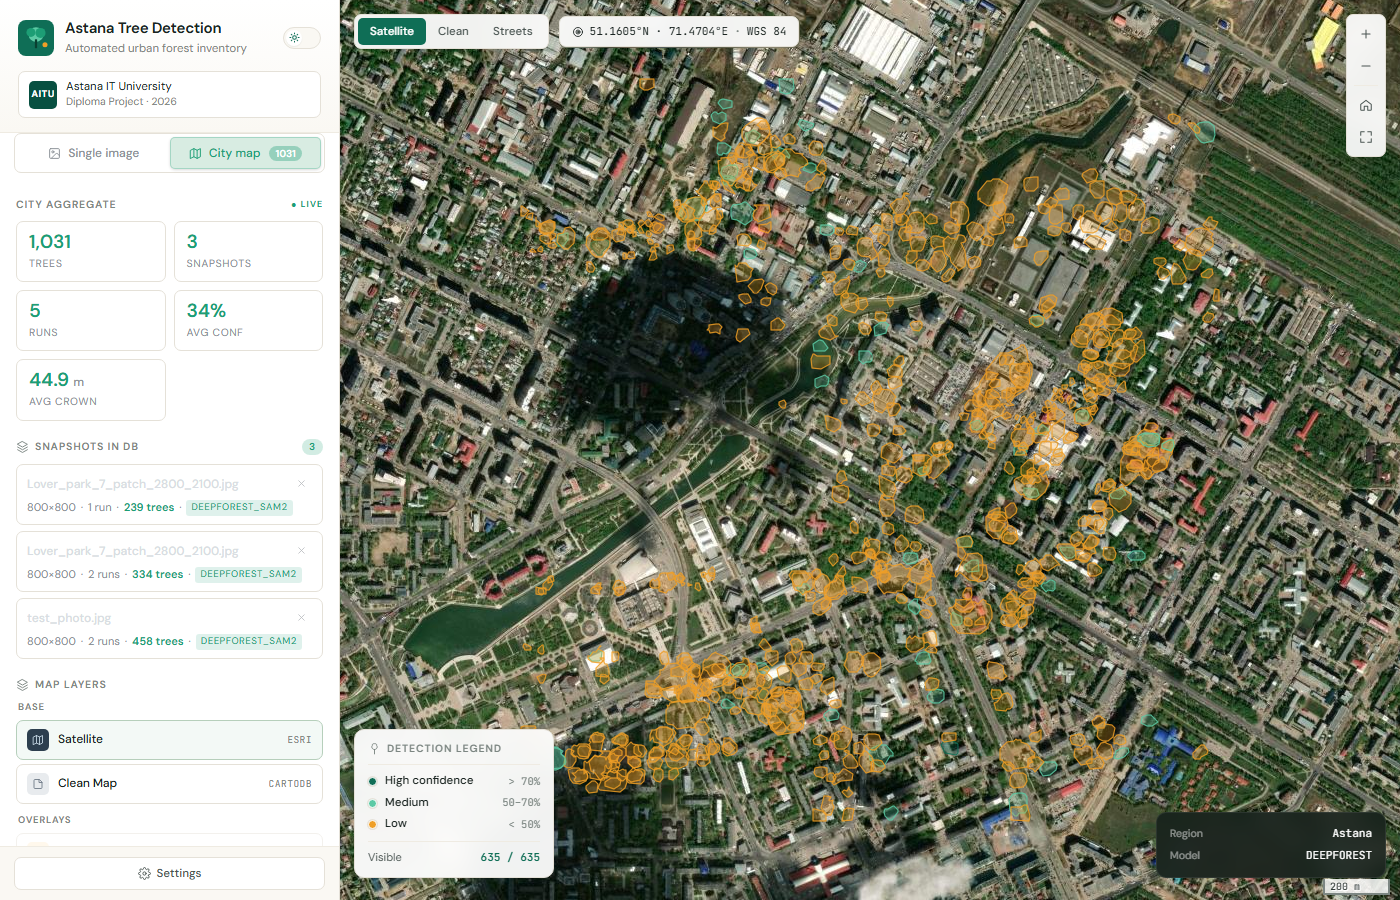
\includegraphics[keepaspectratio,alt={Web application showing the DeepForest + SAM 2 pipeline result on an Astana satellite tile. Each detected tree crown is rendered as a semi-transparent polygon mask derived by SAM 2 from the DeepForest bounding-box prompt, providing precise crown boundary outlines without any domain-specific segmentation training. The city-map view (right) accumulates detections across all processed snapshots.}]{figures/ui_city_map_view.png}}
\caption{\emph{Web application showing the DeepForest + SAM 2 pipeline result on an Astana satellite tile. Each detected tree crown is rendered as a semi-transparent polygon mask derived by SAM 2 from the DeepForest bounding-box prompt, providing precise crown boundary outlines without any domain-specific segmentation training. The city-map view (right) accumulates detections across all processed snapshots.}}
\end{figure}

\section{Ensemble strategies}\label{ensemble-strategies}

The system implements two complementary ensemble strategies described in the following sub-sections. The Weighted-Box-Fusion ensemble of Section 2.8.1 combines a YOLO checkpoint with a DeepForest checkpoint (cross-architecture, addressing the complementary failure modes between an instance-segmenter and a bounding-box-only detector); the cross-YOLO voting ensemble of Section 2.8.2 combines four YOLO checkpoints with each other (within-architecture, addressing per-checkpoint training-time variance and per-checkpoint stadium-roof-style failure modes).

\subsection{Weighted Box Fusion (YOLO + DeepForest)}\label{weighted-box-fusion-yolo-deepforest}

The YOLO and DeepForest branches are trained on the same data but with different network architectures, different patch sizes and different loss formulations. Their errors are therefore partly de-correlated: YOLO tends to over-segment large, dense canopies into several smaller crowns, while DeepForest tends to merge adjacent crowns into a single bounding box. An ensemble that combines the two should benefit from this complementarity.

The chosen ensemble strategy is \textbf{Weighted Box Fusion} {[}26{]}, a recent improvement over the older Non-Maximum-Suppression and Soft-NMS ensembles. Where NMS keeps the single highest-confidence box and discards every overlapping box, WBF instead \textbf{averages} the coordinates of the overlapping boxes weighted by their confidence scores, producing a single fused box whose coordinates and confidence are functions of all the contributing detections.

Formally, for a cluster of \(n\) overlapping predictions \(\{(\mathbf{b}_{i}, c_{i})\}_{i=1}^{n}\), where \(\mathbf{b}_{i} = (x_{1}, y_{1}, x_{2}, y_{2})_{i}\) is the \(i\)-th box and \(c_{i}\) is its confidence, the WBF-fused box and fused confidence are

\[
\mathbf{b}_{\text{fused}} \;=\; \frac{\sum_{i=1}^{n} c_{i}\, \mathbf{b}_{i}}{\sum_{i=1}^{n} c_{i}}, \qquad
c_{\text{fused}} \;=\; \frac{\sum_{i=1}^{n} c_{i}}{n} \cdot \frac{\min(n, M)}{M}
\]

where \(M\) is the total number of models being ensembled (here \(M = 2\), YOLO and DeepForest). The right-hand factor \(\min(n, M)/M\) down-weights clusters that contain detections from only a subset of the available models --- a single-model cluster receives half of its raw average confidence, while a two-model cluster receives the full average. This factor is the key conceptual difference between WBF and a naive confidence-weighted average and is what makes WBF a true ensemble (it rewards agreement between models) rather than a smoothing operation.

The WBF procedure as implemented in the system is:

\begin{enumerate}
\def\labelenumi{\arabic{enumi}.}
\tightlist
\item
  Run the YOLO and DeepForest adapters on the same image and collect the two sets of bounding boxes with their confidence scores.
\item
  Normalise the box coordinates to \([0, 1]\) by dividing by the image dimensions.
\item
  Sort the union of both sets by confidence in decreasing order and process each box in turn: if the current box has IoU \(\geq T_{\text{IoU}}\) with the existing fused box of an already-formed cluster, add it to that cluster; otherwise, start a new cluster with the current box alone.
\item
  After all boxes have been processed, replace each cluster of \(n\) boxes with a single fused box whose coordinates are the confidence-weighted average of the cluster members and whose confidence is the sum of the cluster members' confidences scaled by \(\min(n, \text{models}) / \text{models}\) where \(\text{models} = 2\).
\item
  De-normalise the coordinates back to pixel space and return the result.
\end{enumerate}

The implementation uses the open-source \texttt{ensemble-boxes} package from Roman Solovyev's reference repository. The IoU threshold \(T_{\text{IoU}}\) is set to 0.55, slightly higher than the typical 0.5 used for plain NMS, in order to compensate for the systematic location offset between YOLO and DeepForest boxes (the two networks tend to localise the centre of a crown slightly differently due to their different receptive fields). The per-model weights are set to 1.0 for both branches in the current prototype; an ablation study of weight calibration is reserved for future work.

\subsection{Cross-YOLO voting ensemble (IoU-clustered, K-of-N majority vote)}\label{cross-yolo-voting-ensemble-iou-clustered-k-of-n-majority-vote}

A complementary ensemble strategy that operates \textbf{within} the YOLO family rather than across architectures was added to the system in the late stage of the project, motivated by two observations from Chapter 3: the per-checkpoint training-time variance documented in Section 3.3.9 (sample standard deviation ≈ 0.028 Box mAP@50 across four replicates of the same configuration) and the qualitative cross-checkpoint complementarity discussed in Section 3.7.4 (different YOLO checkpoints with similar aggregate mAP detect substantially different per-detection subsets on the same input). The cross-YOLO ensemble averages out the per-checkpoint variance and discards single-checkpoint hallucinations through a majority-voting rule.

\textbf{Algorithm.} Given \(N\) member YOLO checkpoints, the ensemble (i) runs every member on the input image independently, (ii) pools all \(M\) detections from the \(N\) members into a single flat list tagged by member identity, (iii) clusters the pooled detections by box Intersection-over-Union using a union-find data structure (any two detections with \(\text{IoU} \geq 0.5\) become part of the same cluster), (iv) \textbf{discards any cluster whose detections come from fewer than K distinct member models} (default K = 2), and (v) emits the highest-confidence detection from each surviving cluster as the cluster's representative. The complexity is \(O(N M^2)\), dominated by the pairwise IoU computation rather than the union-find; on a typical Astana tile with M ≈ 750 per member the four-member ensemble runs end-to-end in approximately 4--5 seconds on the laptop GPU. The implementation lives in \texttt{backend/models/yolo\_ensemble\_adapter.py} (\texttt{MultiYOLOEnsembleAdapter}) and an equivalent CLI tool with the same algorithm is provided as \texttt{ml/v5\_ensemble.py}.

\textbf{Default member set.} Four YOLO checkpoints from the project archive are configured as the default ensemble members in the backend, chosen for the visual complementarity of their failure modes on Astana scenes:

\begin{itemize}
\tightlist
\item
  \textbf{v4\_x\_clean} --- the final production checkpoint (Round 4 winner, yolov8x-seg + Ultralytics defaults), strongest aggregate mAP, conservative on built-environment surfaces;
\item
  \textbf{exp1\_m\_cocostart} --- yolov8m-seg with v2-proven augmentation (Round 1 winner), recovers more partially-occluded crowns than v4\_x\_clean;
\item
  \textbf{v4\_s\_clean} --- yolov8s-seg with defaults, the smallest reasonable variant, most permissive (highest raw detection count, useful for recall-priority scenes);
\item
  \textbf{v2-finetune} --- the previous-generation production checkpoint, most conservative on novel surface types (no stadium-roof false-positive regression of the Round 4 / exp1 generation).
\end{itemize}

\textbf{Frontend integration.} The cross-YOLO ensemble is exposed in the frontend's hierarchical model picker under the \textbf{Ensemble → 4× YOLO vote} option (Section 2.11.3 of this chapter). The user can toggle between the WBF ensemble of Section 2.8.1 (cross-architecture: YOLO + DeepForest) and the cross-YOLO ensemble of this section at runtime without restarting the backend.

\section{Geographic conversion}\label{geographic-conversion}

A pixel coordinate \((x, y)\) inside the detection mask has no immediate meaning to a municipal user; the system must convert it into a \((\text{longitude}, \text{latitude})\) pair in WGS-84. The conversion is implemented in \texttt{backend/geo.py} and supports four operating modes, selected automatically by the system depending on the metadata available.

\textbf{Mode 1 --- GeoTIFF affine.} If the input image is a GeoTIFF, the affine transform written in the file's metadata maps any pixel coordinate to a coordinate in the projection of the file. The system reads the transform with \texttt{rasterio.transform.AffineTransformer.xy(row,\ col)} and then re-projects the result to EPSG:4326 with \texttt{pyproj.Transformer} if needed. This mode is the most accurate and is the recommended workflow for production use.

\textbf{Mode 2 --- Four-corner bilinear.} If the user supplies the geographic coordinates of all four corners of the image (typically by dragging four markers on the Leaflet map until the screenshot is aligned with the underlying satellite basemap), the conversion uses bilinear interpolation: for a pixel at relative coordinates \((u, v) \in [0,1]^2\), the geographic position is \[
\mathbf{g}(u,v) = (1-u)(1-v)\mathbf{g}_{\text{nw}} + u(1-v)\mathbf{g}_{\text{ne}} + (1-u)v\mathbf{g}_{\text{sw}} + uv\mathbf{g}_{\text{se}}.
\] This mode is appropriate when the image is a rectified satellite view but the precise corners are not known from EXIF or from a GeoTIFF.

\textbf{Mode 3 --- Two-corner axis-aligned.} When only the north-west and south-east corners are known (the common case after the in-browser map-capture workflow described in section 2.2), the conversion degenerates to a simple linear interpolation along each axis: \[
\lambda(x) = \lambda_{\text{nw}} + (x / W) (\lambda_{\text{se}} - \lambda_{\text{nw}}), \qquad \phi(y) = \phi_{\text{nw}} + (y / H) (\phi_{\text{se}} - \phi_{\text{nw}}).
\] This is exact under the assumption of an axis-aligned, equirectangular projection at the city scale (the meridian curvature is negligible across a few hundred metres of Astana).

\textbf{Mode 4 --- None.} If the user does not supply any geographic information and the input is not a GeoTIFF, the system returns the detections in pixel coordinates only and the corresponding fields of the JSON response are left as \texttt{null}. The Leaflet map is then disabled in the frontend and only the raw detections are displayed.

The choice of mode is recorded in the response metadata so that downstream users can know what level of geographic accuracy to expect.

In addition to the pure coordinate conversion, the geographic module estimates the \textbf{pixel size in metres} at the centre of the image, using the Haversine formula on the image diagonal. The estimated pixel size is propagated through to all downstream statistics --- average crown area in square metres, total green coverage in hectares, total tree count per hectare --- and is reported alongside the inventory.

\section{Result aggregation, persistent storage and export}\label{result-aggregation-persistent-storage-and-export}

After the geographic conversion the system produces a final \texttt{PredictResult} object that contains:

\begin{itemize}
\tightlist
\item
  The job identifier and the originating image identifier.
\item
  The list of detections, each with an integer index, a bounding box in pixel and geographic coordinates, a polygon mask, a confidence score, a crown area in pixels and (if applicable) in square metres.
\item
  The total time taken by the inference, in milliseconds, for performance benchmarking.
\item
  A \texttt{stats} block with the tree count, the mean/min/max confidence, the average crown area, the green-coverage percentage and (when pixel size is known) the analysed area in hectares.
\end{itemize}

\textbf{Persistent storage.} All results are written to a local SQLite database at \texttt{storage/app.db} rather than kept in a Python process dictionary. The schema consists of three tables linked by foreign keys with \texttt{ON\ DELETE\ CASCADE}:

\begin{itemize}
\tightlist
\item
  \texttt{snapshots} --- one row per uploaded or captured image, with file path, geographic bounds and capture metadata;
\item
  \texttt{runs} --- one row per model invocation on a snapshot, with model name, confidence threshold, total inference time and the chosen geographic mode;
\item
  \texttt{detections} --- one row per detected tree, with the bounding box, polygon mask, confidence, crown area and geographic coordinates.
\end{itemize}

The persistence layer is implemented in \texttt{backend/db.py} and is used by every read and write path in the backend. The schema choice has three practical consequences. First, restarting the FastAPI process loses no detections --- a critical property for any tool that is expected to be operated by a non-developer end user. Second, the \textbf{city-map view} (described in Section 2.11 below) can query the database for \emph{every detection ever produced} with a single SQL query and visualise them all on a single Leaflet layer; this is the principal aggregate-inspection workflow of the application. Third, snapshot deletion is implemented via a single \texttt{DELETE\ FROM\ snapshots\ WHERE\ id\ =\ ?} statement; the cascading foreign keys then remove all dependent runs, detections and the source image file from disk.

\textbf{Export.} Three exporters are provided, all sharing a common implementation in \texttt{backend/export.py} and reachable via \texttt{POST\ /api/export/\{job\_id\}/\{format\}}:

\begin{itemize}
\tightlist
\item
  \textbf{GeoJSON} --- a FeatureCollection in which each detection is a single Feature whose geometry is a Polygon (the crown mask in WGS-84) and whose properties contain the confidence, the crown area and the bounding box. The GeoJSON file can be loaded directly into QGIS, ArcGIS or any compatible GIS tool.
\item
  \textbf{CSV} --- a flat table with one row per detection and columns for the index, the centroid coordinates, the bounding box, the confidence and the area. The CSV is intended for spreadsheet-based inspection and for direct ingestion by \emph{Zelenstroy}'s existing reporting workflow.
\item
  \textbf{Standalone HTML} --- a single self-contained HTML file with a Leaflet map embedded inline, the OpenStreetMap and ESRI World Imagery basemaps loaded from CDN, and the detections rendered as a vector layer with on-hover popups. The file is intended for sharing the inventory with a non-technical audience that does not have access to a GIS tool.
\end{itemize}

\section{Frontend application and user workflows}\label{frontend-application-and-user-workflows}

The frontend is a single-page React 18 application served by FastAPI at the root URL, implemented in three files (\texttt{frontend/index.html}, \texttt{frontend/app.jsx}, \texttt{frontend/styles.css}) and a small API client (\texttt{frontend/api.js}). The application deliberately avoids a build step: React, Babel-standalone and Leaflet are loaded directly from a CDN as UMD bundles. The motivation for this choice is operational simplicity --- a municipal employee can run the system without Node.js, npm or any other JavaScript toolchain installed on the host.

\subsection{Two view modes}\label{two-view-modes}

The application exposes two main views, switchable in the sidebar.

\textbf{Single image view} is the workflow for a single satellite image. The user uploads a PNG, JPG or GeoTIFF (or captures one interactively from the map), selects a detection model and a confidence threshold, clicks \emph{Run detection} and watches a progress indicator while the backend performs inference. The result is then visualised in three coordinated panels: a Leaflet map with the image overlaid as a semi-transparent layer and the detections rendered on top; a statistics panel showing the tree count, the green-coverage percentage, the mean confidence and the analysed area in hectares; and a confidence-filter slider that interactively hides or shows low-confidence detections without re-running the model.

\begin{figure}
\centering
\pandocbounded{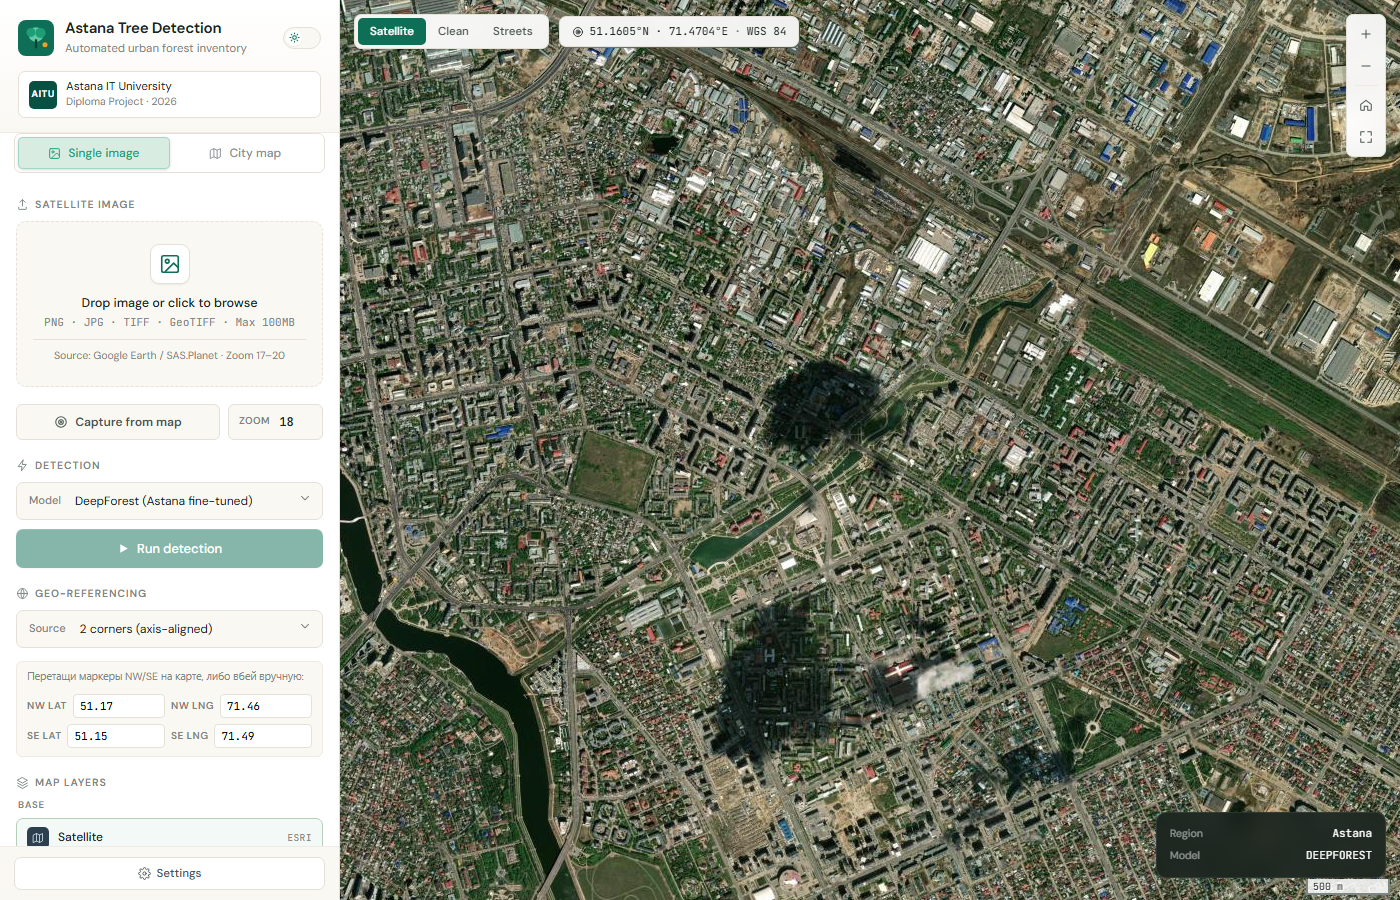
\includegraphics[keepaspectratio,alt={Single-image view of the web application. The left panel shows the satellite image upload zone, model selector dropdown (YOLO / Mask R-CNN / DeepForest / DeepForest+SAM 2 / Ensemble), confidence threshold, four-mode geographic referencing controls and export buttons (GeoJSON, CSV, HTML). The main panel displays the Leaflet satellite basemap with the uploaded image overlay and detected tree crowns rendered as polygon masks.}]{figures/ui_single_image_view.png}}
\caption{\emph{Single-image view of the web application. The left panel shows the satellite image upload zone, model selector dropdown (YOLO / Mask R-CNN / DeepForest / DeepForest+SAM 2 / Ensemble), confidence threshold, four-mode geographic referencing controls and export buttons (GeoJSON, CSV, HTML). The main panel displays the Leaflet satellite basemap with the uploaded image overlay and detected tree crowns rendered as polygon masks.}}
\end{figure}

\begin{figure}
\centering
\pandocbounded{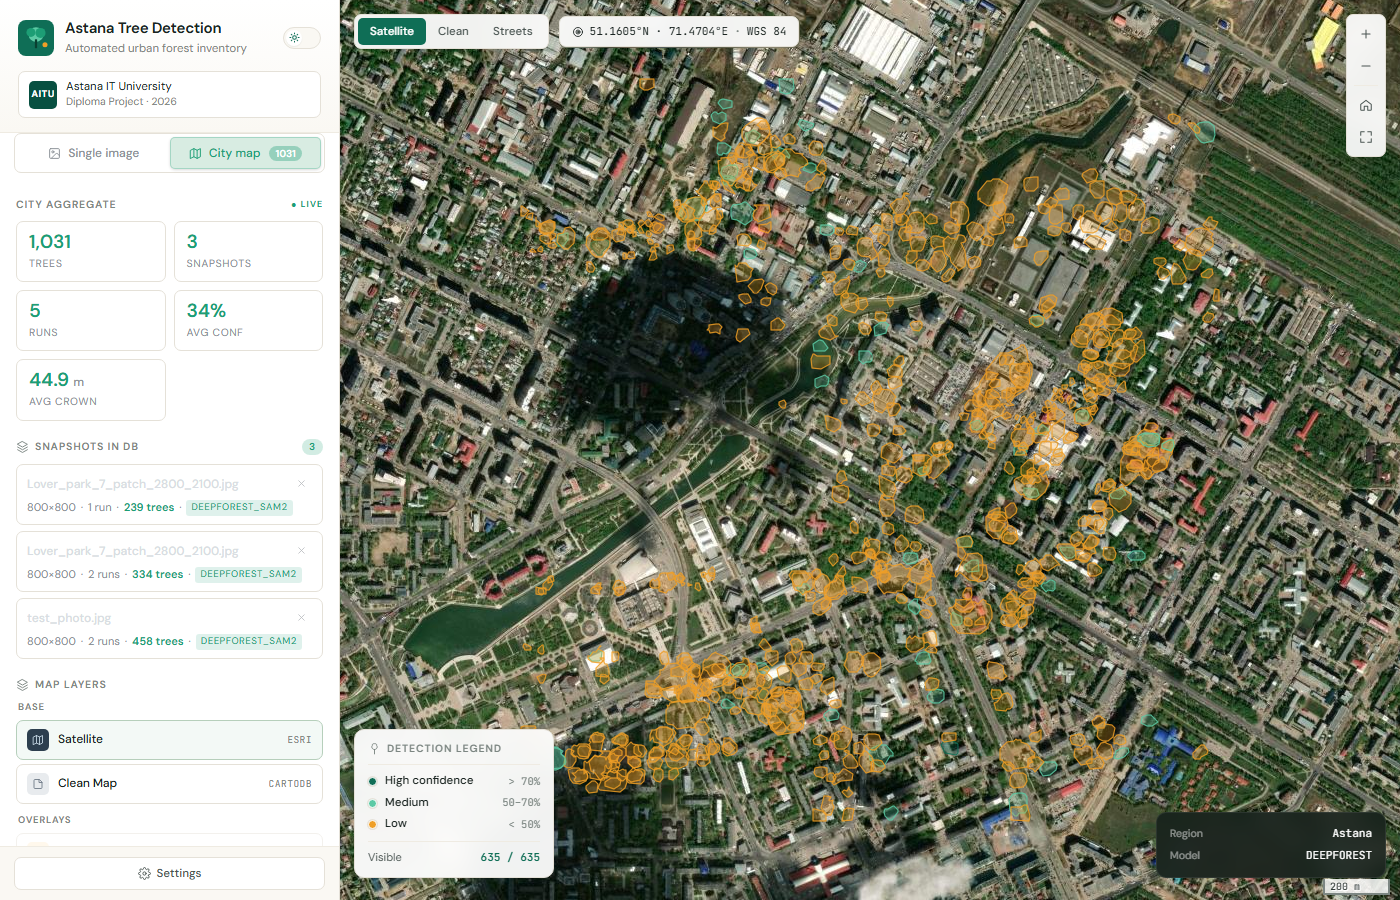
\includegraphics[keepaspectratio,alt={City-map view showing 1 031 detected trees across three processed Astana snapshots. Crown polygons are colour-coded by confidence (green: high ≥ 70 \%, yellow: medium 50--70 \%, red: low \textless{} 50 \%). The left panel shows aggregate statistics and a per-snapshot list. This view is the principal operational deliverable of the system, enabling city-wide tree inventory accumulation over time.}]{figures/ui_city_map_view.png}}
\caption{\emph{City-map view showing 1 031 detected trees across three processed Astana snapshots. Crown polygons are colour-coded by confidence (green: high ≥ 70 \%, yellow: medium 50--70 \%, red: low \textless{} 50 \%). The left panel shows aggregate statistics and a per-snapshot list. This view is the principal operational deliverable of the system, enabling city-wide tree inventory accumulation over time.}}
\end{figure}

\textbf{City-map view} is the aggregate-inspection mode. It queries the persistent database for the full collection of all snapshots ever processed by the system and renders every detected tree on a single Leaflet layer (with a safety cap of 50 000 detections to protect the browser). A side panel lists each snapshot with a per-snapshot summary (number of runs, total trees, last-used model, geographic centre) and a deletion action that cascades through the database and the disk. This view is the principal demonstration deliverable of the project: a single map of Astana that grows tree-by-tree as the user processes new districts, building up an organic city-wide inventory that the user can browse, query, and export at any time.

\subsection{Geographic configuration and Auto-Zoom Region Scan}\label{geographic-configuration-and-auto-zoom-region-scan}

In both views the user controls the geographic mode of the active snapshot through a dedicated panel. The four modes of Section 2.9 are exposed as a segmented switch, and the user can enter corner coordinates either by typing them into form fields or by dragging NW/SE markers directly on the map until the image overlay aligns visually with the basemap; when the user moves a marker, the image overlay is re-bound to the new bounds in real time. The coordinates are written back to the database on the next inference run and persist across page reloads.

The principal map-capture workflow of the application is the \textbf{Auto-Zoom Region Scan}: the user draws a rectangle (or freely-shaped polygon) on the basemap, and the backend automatically subdivides the request into a grid of sub-bounding-boxes at the fixed zoom level of 19 --- the highest available resolution for which the YOLO and DeepForest models were trained --- and processes each sub-region in turn. Three protections combine to keep the operation tractable: a hard cap of nine sub-regions per request (corresponding to approximately a 1.5 × 1.5 km area at zoom 19), the per-sub-region \texttt{MAX\_TILES} cap of Section 2.2, and the use of a streaming NDJSON response on the \texttt{/api/scan\_region/stream} endpoint that lets the frontend show the user incremental progress events (\texttt{plan}, \texttt{capturing}, \texttt{predicting}, \texttt{sub\_complete}, \texttt{done}) as the scan proceeds, rather than blocking on the full operation. Each successful sub-region is persisted as an independent snapshot in the database (Section 2.10) and tagged with the parent scan-session identifier, so a single \texttt{DELETE\ /api/scans/\{id\}} request cascades through all its sub-region snapshots, runs, detections and PNG files in one operation. A polygon-shaped scan additionally applies a \texttt{shapely.Polygon.contains} filter on every detection centroid, retaining only those that fall inside the user-drawn polygon --- useful for inventories of irregular districts, parks or river-front green corridors.

\subsection{Detection display modes and aggregate visualisation}\label{detection-display-modes-and-aggregate-visualisation}

Every detection produced by the backend carries three independent geometric representations: a centre point (latitude / longitude of the bounding-box centroid), an axis-aligned bounding box (four corners in pixel space, lifted into geographic space through the active geo-conversion mode), and a polygon mask (for YOLO, Mask R-CNN and SAM 2-refined branches, a closed sequence of vertices following the projected crown outline). The frontend exposes these as four mutually-exclusive rendering modes through a segmented control: \textbf{Point} (circle at centroid; useful for inspecting density on coarse zoom levels), \textbf{Box} (geographic quadrilateral, important in four-corner geo-mode where the image is rotated relative to north), \textbf{Polygon} (default, projected crown mask) and \textbf{Heat-map} (kernel-density estimate weighted by per-detection confidence via the \texttt{leaflet.heat} plugin, particularly informative on the city-map view at 1 000+ detections where ``hot'' and ``cold'' districts emerge visually). Switching modes is instantaneous and does not require a backend round-trip; when a particular detection lacks data for the currently-selected mode (e.g.~a DeepForest detection without a polygon mask), the frontend falls back automatically to point rendering so the detection never silently disappears from the map.

\subsection{REST endpoints}\label{rest-endpoints}

The backend exposes a complete REST API documented automatically by FastAPI's built-in OpenAPI integration at \texttt{/docs}. Table 2.4 summarises the endpoints used by the frontend and by the export workflows.

\textbf{Table 2.4 --- REST endpoints exposed by the backend.}

{\def\LTcaptype{none} % do not increment counter
\begin{longtable}[]{@{}
  >{\raggedright\arraybackslash}p{(\linewidth - 4\tabcolsep) * \real{0.3333}}
  >{\raggedright\arraybackslash}p{(\linewidth - 4\tabcolsep) * \real{0.3333}}
  >{\raggedright\arraybackslash}p{(\linewidth - 4\tabcolsep) * \real{0.3333}}@{}}
\toprule\noalign{}
\begin{minipage}[b]{\linewidth}\raggedright
Method
\end{minipage} & \begin{minipage}[b]{\linewidth}\raggedright
Path
\end{minipage} & \begin{minipage}[b]{\linewidth}\raggedright
Purpose
\end{minipage} \\
\midrule\noalign{}
\endhead
\bottomrule\noalign{}
\endlastfoot
\texttt{GET} & \texttt{/api/status} & Health check and aggregate counts (snapshots, runs, total trees) \\
\texttt{GET} & \texttt{/api/providers} & List of tile providers with URL templates and max-zoom (used by the frontend to build the provider dropdown and the Leaflet basemap) \\
\texttt{POST} & \texttt{/api/upload} & Upload a satellite image; returns an \texttt{ImageMeta} with assigned id \\
\texttt{POST} & \texttt{/api/capture\_from\_map} & Stitch tiles for \texttt{(nw,\ se,\ zoom,\ provider)} and return an \texttt{ImageMeta} \\
\texttt{POST} & \texttt{/api/scan\_region} & Auto-Zoom Region Scan: subdivide bbox into sub-regions at z = 19, capture + predict each, persist as separate snapshots \\
\texttt{POST} & \texttt{/api/scan\_region/stream} & Same as above with an NDJSON streaming progress response; accepts optional \texttt{polygon} for point-in-polygon filtering \\
\texttt{GET} & \texttt{/api/scans} & List scan-sessions with bbox, zoom, provider, model, sub-region counts, total trees, duration, status \\
\texttt{DELETE} & \texttt{/api/scans/\{id\}} & Cascade-delete a scan-session and all its sub-region snapshots / runs / detections / PNG files \\
\texttt{GET} & \texttt{/api/image/\{id\}} & Serve the raw image PNG \\
\texttt{GET} & \texttt{/api/image/\{id\}/meta} & Image metadata \\
\texttt{POST} & \texttt{/api/predict} & Run inference: \texttt{\{image\_id,\ model,\ confidence,\ geo\}} \\
\texttt{GET} & \texttt{/api/result/\{job\_id\}} & Reload a past prediction result \\
\texttt{GET} & \texttt{/api/snapshots} & List snapshots with per-snapshot aggregates \\
\texttt{GET} & \texttt{/api/detections} & Aggregate query with optional bbox / model / min-confidence filters \\
\texttt{GET} & \texttt{/api/aggregate/stats} & Database-wide summary (counts and averages) \\
\texttt{DELETE} & \texttt{/api/snapshots/\{id\}} & Cascade-delete a snapshot, its runs, its detections and its file \\
\texttt{DELETE} & \texttt{/api/runs/\{job\_id\}} & Delete a single inference run \\
\texttt{POST} & \texttt{/api/export/\{job\_id\}/\{format\}} & Export as GeoJSON / CSV / standalone HTML \\
\texttt{GET} & \texttt{/api/history} & Most recent N runs across all snapshots \\
\end{longtable}
}

The endpoints are intentionally fine-grained: the frontend composes complex views from several small JSON responses rather than from a single monolithic dump, which makes the city-map view efficient even with tens of thousands of detections in the database.

\section{Summary}\label{summary}

This chapter has presented the methodological foundation of the system: a layered architecture in which a thin presentation layer and a stateless REST backend are connected to a pluggable set of four deep-learning model adapters. The four adapters implement complementary detection paradigms --- instance segmentation with YOLOv8-seg (Section 2.4), instance segmentation with Mask R-CNN (Section 2.5), bounding-box detection with DeepForest (Section 2.6), and zero-shot mask refinement with SAM 2 (Section 2.7) --- and the YOLO and DeepForest detector outputs are combined through a Weighted-Box-Fusion ensemble (Section 2.8). Tiled inference allows the system to scale to satellite images of arbitrary resolution; four-mode geographic conversion supports inputs ranging from raw screenshots to fully-georeferenced GeoTIFFs; and three exporters deliver the resulting inventory in formats suitable for GIS specialists, spreadsheet users and non-technical viewers. The next chapter reports the experimental evaluation of the trained models and the integrated system on the Astana dataset.
